\begin{figure*}[tb]
    \centering
    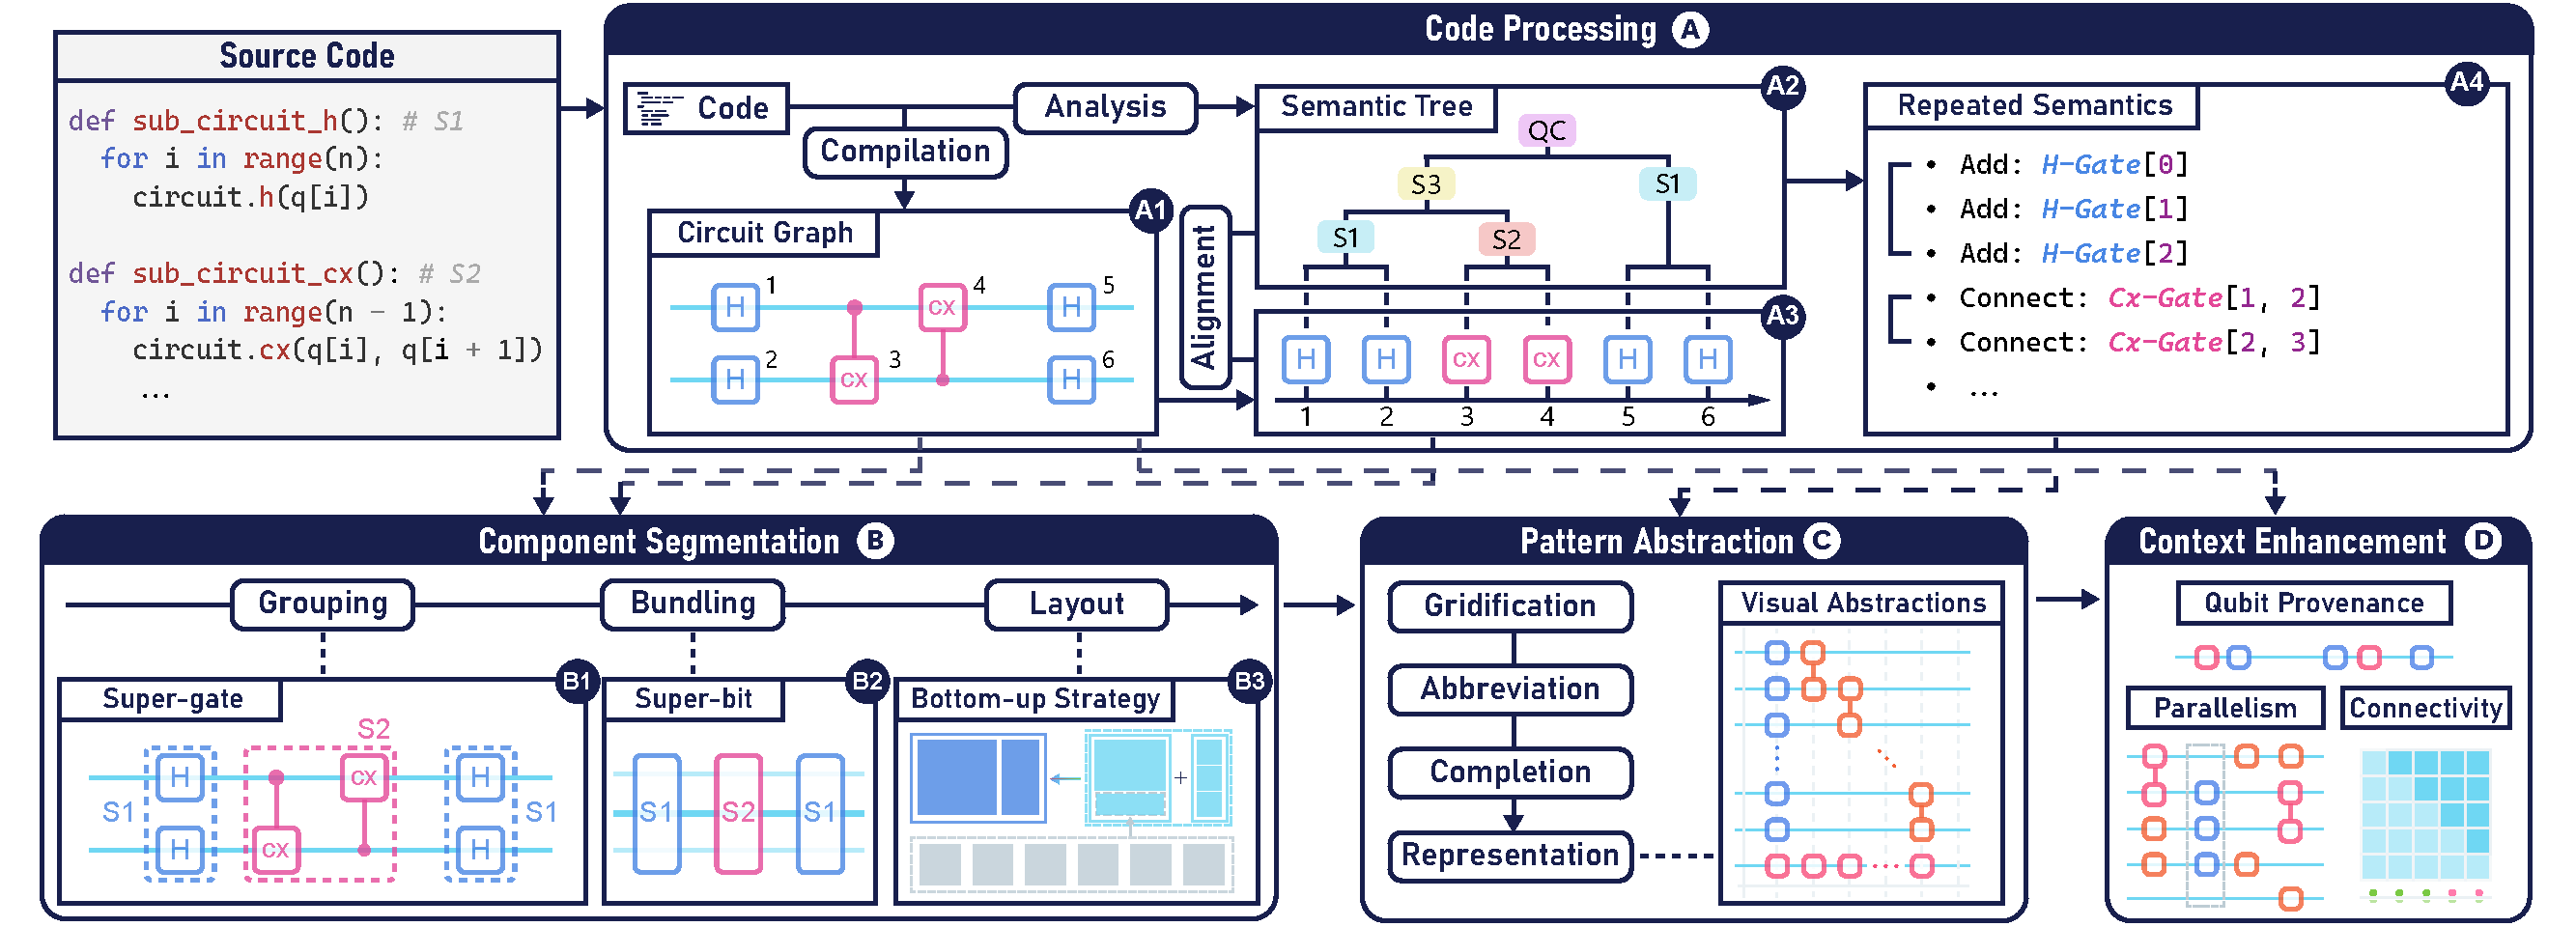
\includegraphics[width=\linewidth]{pipeline-all}
    \caption{%
        The pipeline of our visualization approach comprises four stages.
        (A) We compile and parse the programming code to collect meta-data and semantic information of the quantum circuit.
        (B) Decompose the circuit to hierarchical components with semantic structure.
        (C) Abstract the circuit using visual abstractions of its patterns.
        (D) Enhance the contextual information with a series of visual representations.
    }
    \label{fig:pipeline-all}
\end{figure*}


\section{Visualization Approach}
\label{sec:pipeline}
In this section, we present a pipeline that accepts the programming code of quantum algorithms, 
and results in a series of visual representations to reveal the components ({R1}), patterns ({R2}) and context information ({R3}) of the quantum circuits (\cref{fig:pipeline-all}).
The semantic structure tree of the quantum circuit is introduced to support flexibly-customized experience throughout the visualization pipeline ({R4}).
To prove the concept of our approach, we implement the proposed pipeline for the quantum circuits that are built using Python with \emph{Qiskit} toolkit. 
% In {\cref{sec:discussion}}, we further discussed that our approach can be easily generalized to other programming languages and toolkits.


\subsection{Code Processing}
\label{sec:code}
% To extract the meta-data and latent semantic information of a quantum circuit, 
% we perform circuit compilation and semantic analysis based on the source code (\cref{fig:pipeline-all}-A).
% Then, we employ data alignment to bridge the gap between the data and semantics.
To support the visualization of a quantum circuit, our pipeline first processes its underlying code through circuit compilation, semantic analysis, and data alignment (\cref{fig:pipeline-all}-A).
This process allows us to extract meta-data and semantic information from the circuit.
% The source code of a quantum circuit may contain condition statements, loops, and function calls, which declares the constructing procedure of the circuit.
% The meta-data pertain to the entities of the circuit, while the semantic information denotes the circuit's structure and patterns present within it.
% \hl{Before visualizing a circuit, we first extract its meta-data from the source code (\cref{fig:pipeline-all}-A), which includes the basic information of the quantum circuit model, like qubits, gates and gate execution orders. To further assist the analysis, we also extract semantic information, which reveals the functionalities of different parts of the circuit.}

\textbf{Circuit Compilation.}
We compile the code and extract the following data from the quantum circuit:
(1) the qubits involved in the circuit,
(2) the quantum gates applied in the circuit with their correlations to qubits, and
(3) the placements of quantum gates in the circuit which indicate the order of execution. 
The above data can be translated to the nodes, edges, and the layout of a circuit graph, which could construct a definite quantum circuit diagram as shown in \cref{fig:pipeline-all}-A1.

% \textbf{Semantic information.}

\textbf{Semantic Analysis.}
Two types of semantic information are derived from the source code.
(1) The \emph{semantic structure} of the code implies the hierarchical structure of sub-circuits.
As there are sub-circuit reuses, researchers usually define some frequently-used circuit construction processes as functions, where each function corresponds to a specific functionality.
Thus, the source code is organized as a tree structure where each tree node represents a function (\cref{fig:pipeline-all}-A2).
We extract this structure through an AST.
% Each function that comprises of a set instructions for building gates corresponds to a sub-circuit, \emph{i.e.} a component gate \icon{component}.
% Thus we get a hierarchical structure of the quantum circuit that consists of a series of component gates.
(2) The \emph{semantic meanings} of code provide insights into patterns in the quantum circuit.
We identify three categories of repetitive patterns from loop statements using a rule-based method, which are detailed in \cref{sec:abs-space}.

\textbf{Node Alignment.}
We apply \emph{node alignment} to establish a connection between the quantum gates and the nodes of semantic structure tree.
Applying semantic or syntactic analysis alone is insufficient to establish a precise correspondence between gates and tree nodes.
We thus insert interrupts in the circuit compilation procedure to track the insertion sequence of quantum gates,
and link the newly-built gates to their semantic representations along with the circuit constructing process. \Cref{fig:pipeline-all}-A3 indicates the \emph{time stamp} of each gate and its corresponding tree node.
As a result, all quantum gates are aligned to the semantic tree nodes.
% For example, ${Gate}_i$ is linked to $Node_i$, which is declared in the function \emph{sub\_circuit\_h}.

% Consequently, the aforementioned data are utilized in the subsequent circuit analysis and visualization process.


\subsection{Component Segmentation}
\label{sec:segment}
To incorporate {R1}, we present a three-step approach for breaking down a typical quantum circuit diagram into hierarchical representations (\cref{fig:pipeline-all}-B).
Our approach draws inspiration from techniques such as node grouping and edge bundling that are effective for graph summarization\cite{Liu:2018:GSM}.
Afterwards, a semantic-preserving layout strategy is introduced to arrange the new diagram.

\textbf{Quantum Gate Grouping.}
The semantic tree (\cref{fig:pipeline-all}-A2) is first employed to guide the segmentation of circuit components.
We label attributes on quantum gates based on a user-customized semantic tree.
Before grouping, users can interactively fold or unfold the tree nodes to control the level of detail (\cref{sec:system:interaction}).
Then, all quantum gates will be labeled with two attributes.
(1) \emph{Tree node label}: 
Each gate will be labeled in accord with the nearest unfolded node to which it belongs.
For example, if the tree node $S1$ is folded while $S3$ is unfolded, then ${Gate}_1$ and ${Gate}_2$ would be labeled with $S3$.
(2) \emph{Loop time label}: 
As a tree node may be repeated in compilation due to loops, two groups of gates may correspond to the same tree node.
We thus label each gate with a time stamp to differentiate separated gate groups that are built from the same function.
Subsequently, the gates will be aggregated by attributes to compose super-gates (\cref{fig:pipeline-all}-B1), analogous to a supernode in a summarized graph.
As a result, the quantum circuit is broken down to a series of primitive \icon{singlegate} \icon{multigate} and component \icon{component} gates.

\textbf{Qubit Bundling.}
% Bundle sequential qubits with the same path hashing.
For a circuit with hundreds of qubits, a typical diagram will display a line for each qubit, which causes massive overlaps when displaying multi-qubit gates.
% A bundled gates involves a number of duplicated wires \icon{qubit} between connected component gates \icon{component}, which may result in visual clutter.
An effective solution to alleviate the problem is adopting the edge bundling technique\cite{Holten:2006:HEB} for combining neighboring edges.
However, the classic method needs to be modified for the quantum circuit.
Due to the fact that each wire represents a distinct qubit throughout the whole circuit,
solely sharing end nodes within a local scope is not a sufficient reason to bundle two qubits together.
They may play a different role in other portions of the circuit.
Therefore, the bundled qubits must be contiguous and of the same provenance throughout the circuit.
The same provenance means these qubits go through the same sequence of primitive or component gates.
For example, all the qubits in \cref{fig:pipeline-all}-B2 go through $S1 \rightarrow S2 \rightarrow S1$, so they can be bundled as one super-bit.


\textbf{Layout Strategy.}
Since the grouping and bundling process breaks up the placements of quantum gates, we present a {bottom-up} layout strategy to reorganize the placements with minimum circuit length and maximum semantic-preserving.
First, we order the sequence of gates by their insertion time stamps (\cref{fig:pipeline-all}-A3). 
The time stamp of the primitive gates \icon{singlegate} \icon{multigate} has been calculated in the \emph{node alignment} process (\cref{sec:code}).
On this basis, the time stamp of the component gate \icon{component} is retrieved from its sub-components.
Secondly, we arrange the layout referring to the semantic structure from the bottom to the top.
The gates in the same tree node are arranged in a local circuit space following the order of their time stamp.
They are laid out on the left most idle place of its correlated qubit wires \icon{qubit} to compress the length of circuit.
If two gates are intersected at the same column, the later gate would be moved backward.
Subsequently, the local layouts of sibling tree nodes will be concatenated while calculating layout for their parent node.
In this way, we could construct a layout from the bottom to the top that shortens circuit length and preserves the semantic structure.



\subsection{Pattern Abstraction}
\label{sec:pattern-abs}
{\tname} abstracts patterns of quantum gates to simplify the representation of the quantum circuit ({R2}).
The pattern of quantum gates refers to the composition and repetition paradigm in a sub-circuit.
However, the composition of the circuit has been explicitly outlined through the component segmentation approach ({\cref{sec:segment}}).
Therefore, we focus on visual abstractions of repeated patterns in this phase.

\subsubsection{Abstraction Space}
\label{sec:abs-space}
Based on a survey of {18} benchmarks of quantum algorithms and expert interviews, we distilled common patterns and abstraction designs of quantum circuits.
The classification and visual representations for these patterns are summarized in \cref{fig:abs-design}.

% \textbf{Directional Repetition Abstraction.}
The statistic result demonstrates that repetitions are necessary patterns in the design of scalable quantum circuits (\cref{fig:abs-design}-A).
% Directional repetitions appear in all 16 benchmarks (15-vertical, 9-horizontal, 9-diagonal).
One observation is that researchers utilize loop statements to repeat sub-circuits for creating scalable circuit.
The repeated sub-circuits are represented as periodic visual patterns in the general quantum circuit diagrams.
We categorize these repetitions owing to their direction, including \emph{vertical}, \emph{horizontal}, and \emph{diagonal} repetitions (\cref{fig:abs-design}-B).


% \begin{itemize}[leftmargin=10pt, noitemsep]
%     \item
\setlength{\intextsep}{0pt}
\setlength{\columnsep}{2pt}
\begin{wrapfigure}{l}{0.5cm}
    \centering 
    
\includegraphics[height=0.5cm]{ver-rep} 
\end{wrapfigure}
\noindent
    % When applying the same operation on a sequence of qubits simultaneously, it is shown as a vertical repetition.
    \emph{\underline{Vertical Repetition}} describes the application of the same operation on a sequence of qubits simultaneously.
    A typical instance of vertical repetition is applying H-gates on all qubits simultaneously.

    % \item
    % When applying a sequence of similar operations on a qubit continuously, it is shown as a horizontal repetition.
\setlength{\intextsep}{0pt}
\setlength{\columnsep}{2pt}
\begin{wrapfigure}{l}{0.5cm}
    \centering 
    
\includegraphics[height=0.5cm]{hor-rep} 
\end{wrapfigure}
\noindent
    \emph{\underline{Horizontal Repetition}} presents a sequence of similar operations applied continuously on a single qubit.
    An example of horizontal repetition is applying a series of Rz-gates on the same qubit.

    % \item
\setlength{\intextsep}{0pt}
\setlength{\columnsep}{2pt}
\begin{wrapfigure}{l}{0.5cm}
    \centering 
    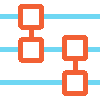
\includegraphics[height=0.5cm]{dig-rep} 
\end{wrapfigure}
\noindent
    \emph{\underline{Diagonal Repetition}} stands for applying a sequence of end-to-end operations on a series of qubits continuously.
    These gates are shown in stages.
    An example of diagonal repetition is applying a series of Cx-gates one next to another.

% \end{itemize}
% \st{These repetitive operations can be a sub-circuit which is a composition of quantum gates rather than a single gate.}
In abstractions, each repeated sub-circuit is regarded as a group.
To reveal the frequency and the detail of groups, we preserve the first two sub-circuits and the last sub-circuit for each directional repetition, whilst the intermediate units are simplified as dots. 

\begin{figure}[h]%
    \centering
    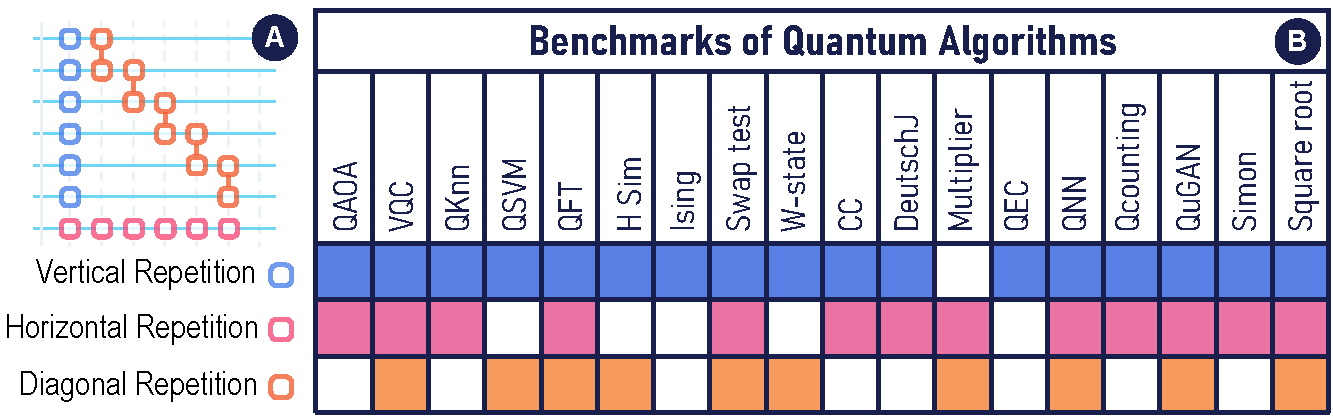
\includegraphics[width=\linewidth]{abstraction-design}
    \caption{%
        Statistics of the pattern occurrence in 18 benchmark quantum algorithms.
        Three commonly repeated patterns are identified in these algorithms: vertical, horizontal, and diagonal repetition.%
    }
    \label{fig:abs-design}
\end{figure}

% \textbf{Data Encoder Abstraction {\color{blue}(Remove)}.}
% A number of quantum algorithms using some specific composition of quantum gates (\emph{e.g.}, \icon{singlegate} or \icon{multigate}) for encoding data features (5/16).
% For example, to solve the MaxCut problem, the QAOA algorithm\cite{Zhou:2020:QAOA} represents edges in a graph by linking qubits with multi-qubit gates \icon{multigate}, where the connected qubits corresponds to the vertices of the edges.
% We categorize the pattern of these data encoder gates as follow:

% % Data link mostly appears in {\color{blue}graph-oriented (x)} benchmarks.
% % It reveals the connectivity of graph data.
% % For example, a fully connected graph results in a circuit in which every qubit is connected to every other qubit.
% \setlength{\intextsep}{0pt}
% \setlength{\columnsep}{2pt}
% \begin{wrapfigure}{l}{0.5cm}
%     \centering 
%     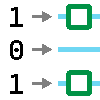
\includegraphics[height=0.5cm]{data-rep} 
% \end{wrapfigure}
% \noindent
% \emph{\underline{Data-dependent Repetition}} indicates iterative gate composition for data encoding.
% \Cref{fig:abs-design}-B4 shows a case of it where a series of Cx-gates is applied on qubit 1 to 6 that encodes a fully-connected graph.

% The data features are represented as uniform but scattered boxes or links on qubit wires \icon{qubit} in the typical quantum circuit diagram, which is inefficient for visual perception.
% As such, we introduce a concise representation to reveal the encoded data features.
% We preserve only one encoder gate in the diagram, and employ a matrix representation to reveal data features ({\color{blue}Figure X}). 

\subsubsection{Abstraction Method}
Our abstraction method effectively abstracts the quantum circuit by selectively highlighting only the necessary components and removing redundant information.
{\Cref{fig:abs-method} depicts an illustration of the procedure.}
This method consists of the following steps:

\noindent
\textbf{STEP1: Gridification.}
We convert the quantum circuit diagram into a series of grids.
Each grid contains exactly one unit box or none.
We assign a visibility attribute to each row and column of the diagram.
A grid is considered visible if its row or column is visible.
Initially, all grids are invisible. 

\noindent
\textbf{STEP2: Abbreviation.}
We identify repetitive patterns in the quantum circuit with the support of semantic meanings extracted from the code, and highlight their start and end parts.
The covered rows and columns are marked as visible.

\noindent
\textbf{STEP3: Completion.}
We iterate through all quantum gates and determine their visibility.
A quantum gate is visible if and only if its connected qubits are all laid on visible grids.

\noindent
\textbf{STEP4: Representation.}
We render all visible gates and aggregate contiguous idle rows and columns. 
Besides, we complement dot marks in the intermediate space of abstractions to improve readability and produce the final representation of the circuit.

% The circuit visualization is converted into $m \times n$ uniform grids, where $m$ indicates the length of the circuit and $n$ denotes the number of qubits.
% Each grid contains exactly one gate or an idle wire.
% We infer the patterns from the semantic information of the source code.

\begin{figure}[h]
    \centering
    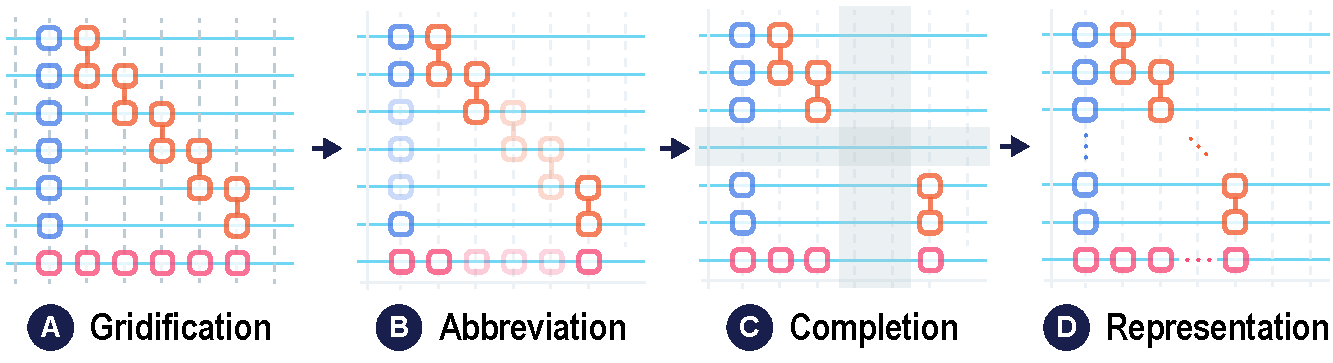
\includegraphics[width=\linewidth]{abs-method}
    \caption{%
        Our abstraction method consists of four steps: (A) gridification, (B) abbreviation, (C) completion, and (D) representation.%
    }
    \label{fig:abs-method}
\end{figure}


\subsection{Context Enhancement}
To provide a contextual perspective of the quantum circuit ({R3}), we extract contextual information from meta-data and utilize a set of visual representations to reveal three factors of interest to domain experts.

\textbf{Qubit Provenance.}
We design a timeline representation for revealing the provenance of each qubit (\cref{fig:context-vis}-A).
All operations applied on the qubit are projected onto the timeline with relative intervals preserved.
% \st{This design facilitates a clear understanding of the genealogy of qubits in the circuit and enables domain experts to trace the origin and evolution of qubits across various stages of the circuit.}
This design enables domain experts to focus on the genealogy of one qubit and trace the evolution across various stages of the circuit.

\textbf{Placement.}
We propose three designs to enhance the visual representation of the quantum circuit and provide contextual information about the placement of quantum gates (\cref{fig:context-vis}-B).
The enhancement involves two aspects: \emph{Parallelism} and \emph{Idle Qubit}.
We first augment the circuit by incorporating color-encoded parallelism levels on the qubit wires (\cref{fig:context-vis}-B1).
Specifically, we assign the color red to indicate heavy-load circuits, while blue denotes light-load circuits.
In addition, the idle spaces around each gate are highlighted to assist in the adjustment of gate placement (\cref{fig:context-vis}-B2). 
The color of the highlighted area represents the idle level.
Notably, when highlighting the idle space for one gate, the idle space of its parallel gates is also highlighted. 
Due to the limitation of screen space, the extent of the idle wire is visualized next to the end of the wires (\cref{fig:context-vis}-B3).
The new diagram reveals the patterns of idling and parallelism in the quantum circuit, which are important factors in understanding and optimizing the performance of the quantum circuit\cite{Bhattacharjee:2017:QCP}. 




\textbf{Connectivity.} 
We employ a matrix-based design to depict the qubit connectivity (\cref{fig:context-vis}-C), 
where a highlighted $cell(i, j)$ indicates a direct connection between the $i$-th and $j$-th qubits via one or multiple multi-qubit quantum gates \icon{multigate}. 
Additionally, we propose a glyph-based design to represent entanglement states. The currently entangled qubits are assigned the same color, while the previous entangled states are visually differentiated and reflected below.
This view provides valuable insights into the overall structure and behavior of the circuit, enabling domain experts to make informed decisions about its optimization.

% Overall, the context enhancement process provides a visual and comprehensive perspective on the quantum circuit by revealing important context information of interest to domain experts. 
% This can help researchers and practitioners better understand the behavior and performance of the circuit, and ultimately optimize its design and execution.


\begin{figure}[h]
    \centering
    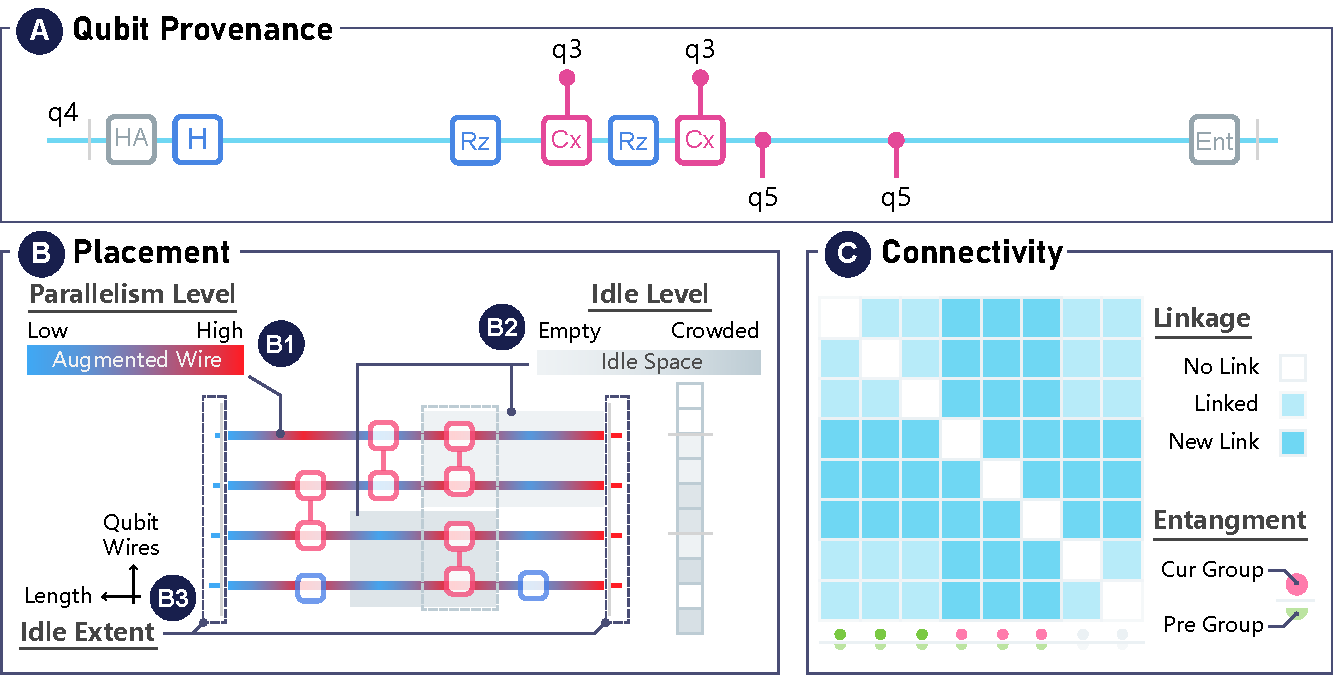
\includegraphics[width=\linewidth]{context-vis}
    \caption{%
        Visual designs of the context visualization.
        (A) The timeline design for qubit provenance.
        (B) The augmented circuit design for quantum gate placement.
        (C) The matrix design for qubit connectivity.
    }
    \label{fig:context-vis}
\end{figure}

